\documentclass[letterpaper,10pt]{book}
% Change to 10 pt
\usepackage{pdfpages}
\usepackage{morewrites}			% to counteract the no write space problem
\setcounter{tocdepth}{6}

\usepackage[framemethod=TikZ]{mdframed}

\usepackage{fancyhdr}

\usepackage{paralist}
\usepackage{amsmath}
\usepackage{amsfonts}
\usepackage{amssymb}
\usepackage{graphicx}

\usepackage{datetime}
%\usepackage{ulem}

%\usepackage[nottoc]{toobibind}

\usepackage[inline]{enumitem}

% Outer margin at 2.50 is exacty correct to fit the ``corruption alert'' tables
\usepackage[inner=1.0in, outer=2.50in, top=2.54cm,bottom=2.54cm, marginparwidth=2.25in]{geometry}

\usepackage{marginnote}
\usepackage{longtable}
\usepackage{booktabs}
\usepackage{xcolor}

\usepackage{soul}

%%%%%%%%%%%%
\definecolor{ForestGreen}{rgb}{0.00,0.29,0.098}
%%%%%%%%%%%%

\usepackage{marginnote}

\usepackage{imakeidx} 
\usepackage[
	backref=true,
	style=numeric,
%	citestyle=numeric,
	backend=bibtex
	]{biblatex}
\usepackage[driverfallback=hypertex,colorlinks=True]{hyperref}
\usepackage{cleveref}

\makeindex[name=scripture,columnsep=20pt, columnseprule=True,columns=3, title=Scripture References]
\makeindex[name=speaker,columnsep=20pt, columnseprule=True,,columns=2, title=Sermon Creator]
\makeindex[name=series,columnsep=20pt, columnseprule=True,,columns=2, title=Sermon Series]
\makeindex[name=date,columnsep=20pt, columnseprule=True,columns=2, title=Sermon Date]
\makeindex[name=event,columnsep=20pt, columnseprule=True,columns=2, title=Event]
\makeindex[name=topic,columnsep=20pt, columnseprule=True,columns=2, title=Topic]
\makeindex[name=AWIP,columnsep=20pt, columnseprule=True,columns=3, title=All Words in Passage]
\makeindex[name=NWIV,columnsep=20pt, columnseprule=True,columns=3, title=Number of Words in Verse]
\makeindex[name=PNIP,columnsep=20pt, columnseprule=True,columns=3, title=Proper Names in Passage]
\makeindex[name=PEIP,columnsep=20pt, columnseprule=True,columns=2, title=Prophetic Events in Passage]
\makeindex[name=TWPAQ,columnsep=20pt, columnseprule=True,columns=1, title=13-Word Phrases and Quotes]
\makeindex[name=PFTTIS,columnsep=20pt, columnseprule=False,columns=3, title=Phrases found 13 times in scripture]
\makeindex[name=WFTTIS,columnsep=20pt, columnseprule=False,columns=3, title=Words found 13 times in scripture]
\makeindex[name=WFITV,columnsep=20pt, columnseprule=False,columns=3, title=Words found in exactly 13 verses]
\makeindex[name=EVENTS,columnsep=20pt, columnseprule=False,columns=2, title=Sermon Log by Place]
\makeindex[name=QUESTIONS,columnsep=20pt, columnseprule=False,columns=2, title=Bible Questions]
\makeindex[name=DOCTRINES,columnsep=20pt, columnseprule=False,columns=2, title=Doctrines]
\makeindex[name=SONGS,columnsep=20pt, columnseprule=False,columns=1, title=Songs]
\makeindex[name=LOCATION,columnsep=20pt, columnseprule=False,columns= 2, title=Location]
\makeindex[name=FACEBOOK,columnsep=20pt, columnseprule=False,columns=2, title=Facebook]
\makeindex[name=DEVOTIONAL,columnsep=20pt, columnseprule=False,columns=2, title=Devotional Items]
%%%%%%%%%%%%%%%%% EXTRA COLORS
\definecolor{champagne}{rgb}{0.97,0.91,0.81}
\definecolor{bone}{rgb}{0.89,0.85,0.79}
\pagestyle{fancy}
\fancyhf{}
\fancyhead[LE,RO]{\today}
\fancyhead[RE,LO]{Daily Bible Reading}
\fancyhead[CE,CO]{-page \thepage  - }

\fancyfoot[CO,CE]{\leftmark}
%\fancyfoot[LE,RO]{CSCE 692, HW1}

\title{DBR\\
Daily \\ Reads}
\author{Keith Anthony \\
\today }
%+/ffffff +   \pagenumbering{gobble}
\bibliography{Bibliographies/All20220122}

\setlength{\fboxsep}{1.0pt}

\usepackage[utf8]{inputenc}
\usepackage{tikz}

\begin{document}
%%%%%%%%%%%% Tile Page

\begin{titlepage}

\begin{flushright}
\rightskip=-2.5cm
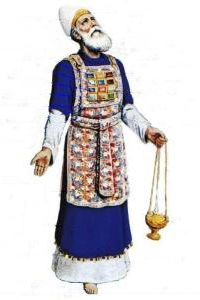
\includegraphics[width=50mm,scale=1.5]{Extras/Melchisedec.jpg}
\vspace{0.4in}  % Create a title for the document and write it in bold font
\LARGE{\textbf{\date}} % Again, do a line break
\linebreak 
% Create a subtitle \large{with Outlines, Statistics, Cross References, and Notes}
\vspace{0.5in}
\begin{flushleft}
\LARGE{Day \#77: Friday, 18  March 2022 PLAIN \\}\vspace{0.25in}
\LARGE{Judges 13-15 Psalm 77 Proverb 18}
\end{flushleft}
\vspace{0.6in}
\bigskip

\normalsize{Xenia, Oh.\\}
\normalsize{created: \today}
\vspace{1.3in}

\end{flushright}
\end{titlepage}

\newpage 
\tableofcontents\hypertarget{TOC}{}
\listoffigures
\listoftables

\hyphenation{A-bim-e-lech bre-thren E-phra-im  Gib-e-o-nites Jer-u-sa-lem through-out Phil-i-stines The-o-phil-us Am-a-le-kites ven-geance Mesh-el-e-mi-ah onan-ism Phar-a-oh thoughts grev-ous-ness Hach-a-liah adul-ter-er Shad-rach}

%%%%%%%%%%%%%%%%% EXTRA COLORS
%%%%%%%%%%%%%%%%% EXTRA COLORS
%%%%%%%%%%%%%%%%% EXTRA COLORS
\definecolor{champagne}{rgb}{0.97,0.91,0.81}
\definecolor{bone}{rgb}{0.89,0.85,0.79}

\definecolor{ForestGreen}{rgb}{0.00,0.29,0.098}
\definecolor{GIVING}{cmyk}{1,0.0,0.72,.1}

\definecolor{MLPE}{cmyk}{1,1,0,.45}
\definecolor{SOCCER}{cmyk}{.77, 0, .42, .49}
\definecolor{PAYBILL}{cmyk}{0,0.83,0.76,0.07}
\definecolor{SERMON}{cmyk}{.14,.9,0,.30} % aka seance \href{http://www.flatuicolorpicker.com/purple-cmyk-color-model/}{seance}
\definecolor{BIBLE}{cmyk}{0,.17,.74,.17}
\definecolor{WORKBLUE}{cmyk}{1, .5, 0, .6}
\definecolor{myOrange}{cmyk}{0, .4, .98, .03}
\definecolor{myTan}{cmyk}{0.0,.07,.17,.10}
\definecolor{myRed}{cmyk}{0,1,1,0}
\definecolor{myWhite}{cmyk}{0,0,0,0}
\definecolor{BLUESoD}{cmyk}{.97,.84,0,.04}
\definecolor{WHITE}{cmyk}{0,0,0,0}
\definecolor{OLDGOLD}{cmyk}{0.05,0.3,1.00,0}
\definecolor{CASTLETON}{cmyk}{1,0,0.31,0.66}
\definecolor{cadmiumgreen}{rgb}{0.0, 0.42, 0.24}
\definecolor{jungle}{rgb}{0.203,0.4882,0.1718}
\definecolor{MYGOLD}{rgb}{1,.84,0}

\definecolor{MYLIGHTGRAY}{rgb}{.85,.85,.85}

\definecolor{codegreen}{rgb}{0,0.6,0}
\definecolor{codegray}{rgb}{0.5,0.5,0.5}
\definecolor{codepurple}{rgb}{0.58,0,0.82}
\definecolor{backcolour}{rgb}{0.95,0.95,0.92}


\mdfdefinestyle{MyFrame}{%
    linecolor=blue,
    outerlinewidth=2pt,
    roundcorner=5pt,
    innertopmargin=\baselineskip,
    innerbottommargin=\baselineskip,
    innerrightmargin=10pt,
    innerleftmargin=10pt,
    backgroundcolor=gray!25!white}


\mdfdefinestyle{MyFrame2}{%
    linecolor=black,
    outerlinewidth=2pt,
    roundcorner=5pt,
    innertopmargin=\baselineskip,
    innerbottommargin=\baselineskip,
    innerrightmargin=10pt,
    innerleftmargin=10pt,
    backgroundcolor=yellow!25!white}


%%%%%
%% for PFTTIS list
%%%%%

%%% And Joseph said unto
\index[PFTTIS]{And Joseph said unto!Genesis!Gen 40:008}
\index[PFTTIS]{And Joseph said unto!Genesis!Gen 40:012}
\index[PFTTIS]{And Joseph said unto!Genesis!Gen 41:025}
\index[PFTTIS]{And Joseph said unto!Genesis!Gen 42:014}
\index[PFTTIS]{And Joseph said unto!Genesis!Gen 42:018}
\index[PFTTIS]{And Joseph said unto!Genesis!Gen 44:015}
\index[PFTTIS]{And Joseph said unto!Genesis!Gen 45:003}
\index[PFTTIS]{And Joseph said unto!Genesis!Gen 45:004}
\index[PFTTIS]{And Joseph said unto!Genesis!Gen 46:031}
\index[PFTTIS]{And Joseph said unto!Genesis!Gen 48:009}
\index[PFTTIS]{And Joseph said unto!Genesis!Gen 48:018}
\index[PFTTIS]{And Joseph said unto!Genesis!Gen 50:019}
\index[PFTTIS]{And Joseph said unto!Genesis!Gen 50:024}


%%% a shadow
\index[PFTTIS]{a shadow!1Chronicles!1Chr 029:15}
\index[PFTTIS]{a shadow!Job!Job 008:09}
\index[PFTTIS]{a shadow!Job!Job 014:02}
\index[PFTTIS]{a shadow!Job!Job 017:07}
\index[PFTTIS]{a shadow!Psalm!Psa 102:011}
\index[PFTTIS]{a shadow!Psalm!Psa 144:004}
\index[PFTTIS]{a shadow!Ecclesiastes!Eccl 006:012}
\index[PFTTIS]{a shadow!Ecclesiastes!Eccl 008:013}
\index[PFTTIS]{a shadow!Isaiah!Isa 04:006}
\index[PFTTIS]{a shadow!Isaiah!Isa 25:004}
\index[PFTTIS]{a shadow!Jonah!Jnh 04:06}
\index[PFTTIS]{a shadow!Colossians!Col 02:017}
\index[PFTTIS]{a shadow!Hebews!Heb 10:001}

%%% blessed is the man
\index[PFTTIS]{blessed is the man!Psalm!Psa 001:001}
\index[PFTTIS]{blessed is the man!Psalm!Psa 032:002}
\index[PFTTIS]{blessed is the man!Psalm!Psa 034:008}
\index[PFTTIS]{blessed is the man!Psalm!Psa 065:004}
\index[PFTTIS]{blessed is the man!Psalm!Psa 084:005}
\index[PFTTIS]{blessed is the man!Psalm!Psa 084:012}
\index[PFTTIS]{blessed is the man!Psalm!Psa 094:012}
\index[PFTTIS]{blessed is the man!Psalm!Psa 112:001}
\index[PFTTIS]{blessed is the man!Proverbs!Pro 008:034}
\index[PFTTIS]{blessed is the man!Isaiah!Isa 056:002}
\index[PFTTIS]{blessed is the man!Jeremiah!Jer 017:007}
\index[PFTTIS]{blessed is the man!Romans!Rom 004:008}
\index[PFTTIS]{blessed is the man!James!Jam 001:012}


%%% carry them
\index[PFTTIS]{carry them!Leviticus!Lev 14:045}
\index[PFTTIS]{carry them!Numbers!Num 11:012}
\index[PFTTIS]{carry them!Joshua!Jsh 04:003}
\index[PFTTIS]{carry them!1Samuel!1Sam 20:040}
\index[PFTTIS]{carry them!1Kings!1Kng 08:046}
\index[PFTTIS]{carry them!2Chronicles!2Chr 06:036}
\index[PFTTIS]{carry them!Ezra!Ezra 05:015}
\index[PFTTIS]{carry them!Isaiah!Isa 40:011}
\index[PFTTIS]{carry them!Isaiah!Isa 41:016}
\index[PFTTIS]{carry them!Isaiah!Isa 57:013}
\index[PFTTIS]{carry them!Jeremiah!Jer 20:004}
\index[PFTTIS]{carry them!Jeremiah!Jer 20:005}
\index[PFTTIS]{carry them!Jeremiah!Jer 43:012}


\index[PFTTIS]{good tidings!2Samuel!2Sam 18:027}
\index[PFTTIS]{good tidings!1Kings!1Ki 01:042}
\index[PFTTIS]{good tidings!2Kings!2Ki 07:009 (2x)}
\index[PFTTIS]{good tidings!Isaiah!Isa 40:009 (2x)}
\index[PFTTIS]{good tidings!Isaiah!Isa 41:007}
\index[PFTTIS]{good tidings!Isaiah!Isa 52:007}
\index[PFTTIS]{good tidings!Isaiah!Isa 61:001}
\index[PFTTIS]{good tidings!Nahum!Nah 01:005}
\index[PFTTIS]{good tidings!Luke!Lk 02:010}
\index[PFTTIS]{good tidings!1Thessalonians!1Thess 03:006}


%%% dead body
\index[PFTTIS]{dead body!Leviticus!Lev 21:011}
\index[PFTTIS]{dead body!Numbers!Num 06:006}
\index[PFTTIS]{dead body!Numbers!Num 09:006}
\index[PFTTIS]{dead body!Numbers!Num 09:007}
\index[PFTTIS]{dead body!Numbers!Num 09:010}
\index[PFTTIS]{dead body!Numbers!Num 09:011}
\index[PFTTIS]{dead body!Numbers!Num 09:013}
\index[PFTTIS]{dead body!Numbers!Num 09:016}
\index[PFTTIS]{dead body!2Kings!2Ki 08:005}
\index[PFTTIS]{dead body!Isaiah!Isa 26:019}
\index[PFTTIS]{dead body!Jeremiah!Jer 26:023}
\index[PFTTIS]{dead body!Jeremiah!Jer 36:030}
\index[PFTTIS]{dead body!Haggai!Hag 02:013}

%%% great sea
\index[PFTTIS]{great sea!Numbers!Num 34:006}
\index[PFTTIS]{great sea!Numbers!Num 34:007}
\index[PFTTIS]{great sea!Joshua!Jos 01:004}
\index[PFTTIS]{great sea!Joshua!Jos 09:001}
\index[PFTTIS]{great sea!Joshua!Jos 15:012}
\index[PFTTIS]{great sea!Joshua!Jos 15:047}
\index[PFTTIS]{great sea!Joshua!Jos 23:004}
\index[PFTTIS]{great sea!Ezekiel!Eze 47:010}
\index[PFTTIS]{great sea!Ezekiel!Eze 47:015}
\index[PFTTIS]{great sea!Ezekiel!Eze 47:019}
\index[PFTTIS]{great sea!Ezekiel!Eze 47:020}
\index[PFTTIS]{great sea!Ezekiel!Eze 48:028}
\index[PFTTIS]{great sea!Daniel!Dan 07:002}


%%% have forsaken me
\index[PFTTIS]{have forsaken me!Judges!Jdg 10:013}
\index[PFTTIS]{have forsaken me!1Samuel!1Sam 08:008}
\index[PFTTIS]{have forsaken me!1Kings!1Ki 11:033}
\index[PFTTIS]{have forsaken me!2Kings!2Ki 22:017}
\index[PFTTIS]{have forsaken me!2Chronicles!2Chr 12:005}
\index[PFTTIS]{have forsaken me!2Chronicles!2Chr 34:025}
\index[PFTTIS]{have forsaken me!Jeremiah!Jer 01:016}
\index[PFTTIS]{have forsaken me!Jeremiah!Jer 02:013}
\index[PFTTIS]{have forsaken me!Jeremiah!Jer 05:007}
\index[PFTTIS]{have forsaken me!Jeremiah!Jer 05:019}
\index[PFTTIS]{have forsaken me!Jeremiah!Jer 16:011 (2x)}
\index[PFTTIS]{have forsaken me!Jeremiah!Jer 19:004}

%%% no king
\index[PFTTIS]{no king!Judges!Jdg 17:06}
\index[PFTTIS]{no king!Judges!Jdg 18:01}
\index[PFTTIS]{no king!Judges!Jdg 19:01}
\index[PFTTIS]{no king!Judges!Jdg 21:25}
\index[PFTTIS]{no king!1Kings!1Ki 22:47}
\index[PFTTIS]{no king!2Kings!2Ki 23:25}
\index[PFTTIS]{no king!Nehemiah!Neh 13:26}
\index[PFTTIS]{no king!Psalms!Psa 033:016}
\index[PFTTIS]{no king!Proverbs!Pro 30:27}
\index[PFTTIS]{no king!Daniel!Dan 02:10}
\index[PFTTIS]{no king!Hosea!Hos 10:03}
\index[PFTTIS]{no king!Micah!Mic 04:09}
\index[PFTTIS]{no king!John!Jhn 19:15}


%%% rebellious house
\index[PFTTIS]{rebellious house!Exodus!Exo 02:005}
\index[PFTTIS]{rebellious house!Exodus!Exo 02:006}
\index[PFTTIS]{rebellious house!Exodus!Exo 02:008}
\index[PFTTIS]{rebellious house!Exodus!Exo 03:009}
\index[PFTTIS]{rebellious house!Exodus!Exo 03:026}
\index[PFTTIS]{rebellious house!Exodus!Exo 03:027}
\index[PFTTIS]{rebellious house!Exodus!Exo 12:002 (2x)}
\index[PFTTIS]{rebellious house!Exodus!Exo 12:003}
\index[PFTTIS]{rebellious house!Exodus!Exo 12:009}
\index[PFTTIS]{rebellious house!Exodus!Exo 12:025}
\index[PFTTIS]{rebellious house!Exodus!Exo 17:012}
\index[PFTTIS]{rebellious house!Exodus!Exo 24:003}

%%% seek him
\index[PFTTIS]{seek him!Deuteronomy!Deu 04:029}\index[PFTTIS]{seek him!1Samuel!1Sam 23:025}
\index[PFTTIS]{seek him!1Chronicles!1Chr 28:009}
\index[PFTTIS]{seek him!2Chronicles!1Chr 15:002}
\index[PFTTIS]{seek him!Ezra!Ezr 08:022}
\index[PFTTIS]{seek him!Psalms!Psa 022:026}
\index[PFTTIS]{seek him!Psalms!Psa 024:006}
\index[PFTTIS]{seek him!Psalms!Psa 119:002}
\index[PFTTIS]{seek him!SoS!SoS 03:002}
\index[PFTTIS]{seek him!SoS!SoS 06:001}
\index[PFTTIS]{seek him!Hosea!Hos 07:010}
\index[PFTTIS]{seek him!Amos!Amo 05:008}
\index[PFTTIS]{seek him!Hebrews!Heb 11:0063}


%%% seek ye
\index[PFTTIS]{seek ye!Isaiah!Isa 34:016}
\index[PFTTIS]{seek ye!Isaiah!Isa 45:019}
\index[PFTTIS]{seek ye!Isaiah!Isa 55:006}
\index[PFTTIS]{seek ye!Amos!Amos 5:004}
\index[PFTTIS]{seek ye!John!John 1:38}
\index[PFTTIS]{seek ye!John!John 18:4}
\index[PFTTIS]{seek ye!John!John 18:7}
\index[PFTTIS]{seek ye!Matthew!Matt 6:33}
\index[PFTTIS]{seek ye!Numbers!Num 16:10}
\index[PFTTIS]{seek ye!Luke!Luke 12:31}
\index[PFTTIS]{seek ye!Luke!Luke 24:5}
\index[PFTTIS]{seek ye!Psalm!Psa 27:8}
\index[PFTTIS]{seek ye!Zephaniah!Zeph 2:3}

%%% the uncircumcised
\index[PFTTIS]{the uncircumcised!Genesis!Gen 17:014}
\index[PFTTIS]{the uncircumcised!Judges!Jdg 14:003}
\index[PFTTIS]{the uncircumcised!Judges!Jdg 15:018}
\index[PFTTIS]{the uncircumcised!2Samuel!2Sam 01:020}
\index[PFTTIS]{the uncircumcised!Isaiah!Isa 02:001}
\index[PFTTIS]{the uncircumcised!Jeremiah!Jer 09:025}
\index[PFTTIS]{the uncircumcised!Ezekiel!Eze 28:010}
\index[PFTTIS]{the uncircumcised!Ezekiel!Eze 31:018}
\index[PFTTIS]{the uncircumcised!Ezekiel!Eze 32:019}
\index[PFTTIS]{the uncircumcised!Ezekiel!Eze 32:027}
\index[PFTTIS]{the uncircumcised!Ezekiel!Eze 32:028}
\index[PFTTIS]{the uncircumcised!Ezekiel!Eze 32:029}
\index[PFTTIS]{the uncircumcised!Ezekiel!Eze 32:032}

%%% worship him
\index[PFTTIS]{worship him!Psalms!Psa 97:007}
\index[PFTTIS]{worship him!Zephaniah!Zeph 02:011}
\index[PFTTIS]{worship him!Matthew!Matt 02:002}
\index[PFTTIS]{worship him!Matthew!Matt 02:008}
\index[PFTTIS]{worship him!John!John 04:023}
\index[PFTTIS]{worship him!John!John 04:024 (2x)} 
\index[PFTTIS]{worship him!Acts!Acts 17:023}
\index[PFTTIS]{worship him!Hebrews!Heb 01:006}
\index[PFTTIS]{worship him!Revelation!Rev 04:010}
\index[PFTTIS]{worship him!Revelation!Rev 13:008}
\index[PFTTIS]{worship him!Revelation!Rev 14:007}
\index[PFTTIS]{worship him!Revelation!Rev 19:010}


%%%%%
%% for PFTTIS list
%%%%%

%%% afflictions
\index[WFTTIS]{afflictions!Psalms!Psa 34:019}
\index[WFTTIS]{afflictions!Psalms!Psa 132:001}
\index[WFTTIS]{afflictions!Acts!Acts 07:010}
\index[WFTTIS]{afflictions!Acts!Acts 20:023}
\index[WFTTIS]{afflictions!2Corinthians!2Cor 06:004}
\index[WFTTIS]{afflictions!Colossians!Col 01:024}
\index[WFTTIS]{afflictions!1Thessalonians!1Thess 03:003}
\index[WFTTIS]{afflictions!2Timothy!2Tim 01:008}
\index[WFTTIS]{afflictions!2Timothy!2Tim 03:011}
\index[WFTTIS]{afflictions!2Timothy!2Tim 04:005}
\index[WFTTIS]{afflictions!Hebrews!Heb 10:032}
\index[WFTTIS]{afflictions!Hebrews!Heb 10:033}
\index[WFTTIS]{afflictions!1Peter!1Pet 05:009}

%%% acsend
\index[WFTTIS]{acsend!Joshua!Jos 06:05}
\index[WFTTIS]{acsend!Psalm!Psa 024:003}
\index[WFTTIS]{acsend!Psalm!Psa 135:007}
\index[WFTTIS]{acsend!Psalm!Psa 139:008}
\index[WFTTIS]{acsend!Isaiah!Isa 14:013}
\index[WFTTIS]{acsend!Isaiah!Isa 14:014}
\index[WFTTIS]{acsend!Jeremiah!Jer 10:013}
\index[WFTTIS]{acsend!Jeremiah!Jer 51:016}
\index[WFTTIS]{acsend!Ezekiel!Eze 38:009}
\index[WFTTIS]{acsend!John!John 06:062}
\index[WFTTIS]{acsend!John!John 20:017}
\index[WFTTIS]{acsend!Romans!Rom 10:006}
\index[WFTTIS]{acsend!Revelation!Rev 17:008}

%%% Assyrian
\index[WFTTIS]{Assyrian!Isaiah!Isa 10:005}
\index[WFTTIS]{Assyrian!Isaiah!Isa 10:024}
\index[WFTTIS]{Assyrian!Isaiah!Isa 14:025}
\index[WFTTIS]{Assyrian!Isaiah!Isa 19:023}
\index[WFTTIS]{Assyrian!Isaiah!Isa 23:013}
\index[WFTTIS]{Assyrian!Isaiah!Isa 30:031}
\index[WFTTIS]{Assyrian!Isaiah!Isa 31:008}
\index[WFTTIS]{Assyrian!Isaiah!Isa 52:004}
\index[WFTTIS]{Assyrian!Ezekiel!Eze 31:003}
\index[WFTTIS]{Assyrian!Hosea!Hos 05:013}
\index[WFTTIS]{Assyrian!Hosea!Hos 11:005}
\index[WFTTIS]{Assyrian!Micah!Hos 05:005}
\index[WFTTIS]{Assyrian!Micah!Hos 05:006}

%%% blot
\index[WFTTIS]{blot!Exodus!Exo 32:032}
\index[WFTTIS]{blot!Exodus!Exo 32:033}
\index[WFTTIS]{blot!Numbers!Num 05:026}
\index[WFTTIS]{blot!Deuteronomy!Deut 09:014}
\index[WFTTIS]{blot!Deuteronomy!Deut 25:019}
\index[WFTTIS]{blot!Deuteronomy!Deut 29:020}
\index[WFTTIS]{blot!2Kings!2Ki 14:027}
\index[WFTTIS]{blot!Job!Job 31:007}
\index[WFTTIS]{blot!Psalms!Psa 51:001}
\index[WFTTIS]{blot!Psalms!Psa 51:009}
\index[WFTTIS]{blot!Proverbs!Pro 09:007}
\index[WFTTIS]{blot!Jeremiah!Jer 18:023}
\index[WFTTIS]{blot!Revelation!Rev 03:005}


%%% chain
\index[WFTTIS]{chain!Genesis!Gen 41:042}
\index[WFTTIS]{chain!1Kings!1Ki 07:017}
\index[WFTTIS]{chain!Psalms!Psa 73:006}
\index[WFTTIS]{chain!SoS!Sos 04:009}
\index[WFTTIS]{chain!Lamentations!Lam 03:007}
\index[WFTTIS]{chain!Ezekiel!Eze 07:023}
\index[WFTTIS]{chain!Ezekiel!Eze 16:011}
\index[WFTTIS]{chain!Daniel!Dan 05:007}
\index[WFTTIS]{chain!Daniel!Dan 05:016}
\index[WFTTIS]{chain!Daniel!Dan 05:029}
\index[WFTTIS]{chain!Acts!Acts 28:020}
\index[WFTTIS]{chain!2Timothy!2Tim 01:016}
\index[WFTTIS]{chain!Revelation!Rev 20:001}


%%% controversy
\index[WFTTIS]{controversy!Deuteronomy!Deu 17:008}
\index[WFTTIS]{controversy!Deuteronomy!Deu 19:017}
\index[WFTTIS]{controversy!Deuteronomy!Deu 21:005}
\index[WFTTIS]{controversy!Deuteronomy!Deu 25:001}
\index[WFTTIS]{controversy!2Samuel!2Sam 15:002}
\index[WFTTIS]{controversy!Isaiah!Isa 34:008}
\index[WFTTIS]{controversy!Jeremiah!Jer 25:031}
\index[WFTTIS]{controversy!Ezekiel!Eze 44:024}
\index[WFTTIS]{controversy!Hosea!Hos 04:001}
\index[WFTTIS]{controversy!Hosea!Hos 12:002}
\index[WFTTIS]{controversy!Micah!Mic 06:002 (2x)}
\index[WFTTIS]{controversy!1Timothy!1Tim 03:016}


%%% Dagon/Dagon's
\index[WFTTIS]{Dagon!Judges!Jdg 16:023}
\index[WFTTIS]{Dagon!1Samuel!1Sam 05:002 (2x)}
\index[WFTTIS]{Dagon!1Samuel!1Sam 05:003 (2x)}
\index[WFTTIS]{Dagon!1Samuel!1Sam 05:004 (3x)}
\index[WFTTIS]{Dagon!1Samuel!1Sam 05:005 (3x)}
\index[WFTTIS]{Dagon!1Samuel!1Sam 05:007}
\index[WFTTIS]{Dagon!1Chronicles!1Chr 10:010}

%%% disobedient
\index[WFTTIS]{disobedient!1Kings!1Ki 13:026}
\index[WFTTIS]{disobedient!Nehemiah!Neh 09:026}
\index[WFTTIS]{disobedient!Luke!Luke 01:017}
\index[WFTTIS]{disobedient!Acts!Acts 26:019}
\index[WFTTIS]{disobedient!Romans!Rom 01:030}
\index[WFTTIS]{disobedient!Romans!Rom 10:021}
\index[WFTTIS]{disobedient!1Timothy!1Tim 01:009}
\index[WFTTIS]{disobedient!2Timothy!2Tim 03:002}
\index[WFTTIS]{disobedient!Titus!Titus 01:016}
\index[WFTTIS]{disobedient!Titus!Titus 03:003}
\index[WFTTIS]{disobedient!1Peter!1Pet 02:007}
\index[WFTTIS]{disobedient!1Peter!1Pet 02:008}
\index[WFTTIS]{disobedient!1Peter!1Pet 03:020}


%%% doubt
\index[WFTTIS]{doubt!Genesis!Gen 37:033}
\index[WFTTIS]{doubt!Deuteronomy!Deu 28:066}
\index[WFTTIS]{doubt!Job!Job 12:002}
\index[WFTTIS]{doubt!Matthew!Matt 14:031}
\index[WFTTIS]{doubt!Matthew!Matt 21:021}
\index[WFTTIS]{doubt!Mark!Mk 11:023}
\index[WFTTIS]{doubt!Luke!Lk 11:020}
\index[WFTTIS]{doubt!John!Jhn 10:024}
\index[WFTTIS]{doubt!Acts!Acts 02:012}
\index[WFTTIS]{doubt!Acts!Acts 28:004}
\index[WFTTIS]{doubt!1Corinthians!1Cor 09:010}
\index[WFTTIS]{doubt!Galatians!Gal 04:020}
\index[WFTTIS]{doubt!1John!1Jhn 02:019}


%%% dungeon
\index[WFTTIS]{dungeon!Genesis!Gen 40:015}
\index[WFTTIS]{dungeon!Genesis!Gen 41:014}
\index[WFTTIS]{dungeon!Exodus!Exo 12:029}
\index[WFTTIS]{dungeon!Jeremiah!Jer 37:016}
\index[WFTTIS]{dungeon!Jeremiah!Jer 38:006 (2x)}
\index[WFTTIS]{dungeon!Jeremiah!Jer 38:007}
\index[WFTTIS]{dungeon!Jeremiah!Jer 38:009}
\index[WFTTIS]{dungeon!Jeremiah!Jer 38:010}
\index[WFTTIS]{dungeon!Jeremiah!Jer 38:011}
\index[WFTTIS]{dungeon!Jeremiah!Jer 38:013}
\index[WFTTIS]{dungeon!Lamentations!Lam 03:053}
\index[WFTTIS]{dungeon!Lamentations!Lam 03:055}


%%% error
\index[WFTTIS]{error!2Samuel!2Sam 06:007}
\index[WFTTIS]{error!Job!Job 19:004}
\index[WFTTIS]{error!Ecclesiastes!Ecc 05:006}
\index[WFTTIS]{error!Ecclesiastes!Ecc 10:005}
\index[WFTTIS]{error!Isaiah!Isa 32:006}
\index[WFTTIS]{error!Daniel!Dan 06:004}
\index[WFTTIS]{error!Matthew!Matt 27:064}
\index[WFTTIS]{error!Romans!Rom 01:027}
\index[WFTTIS]{error!James!Jam 05:020}
\index[WFTTIS]{error!2Peter!2Pet 02:018}
\index[WFTTIS]{error!2Peter!2Pet 03:017}
\index[WFTTIS]{error!1John!1Jn 04:006}
\index[WFTTIS]{error!Jude!Jude 01:011}

%%% fourish
\index[WFTTIS]{fourish!Psalms!Psa 072:007}
\index[WFTTIS]{fourish!Psalms!Psa 072:016}
\index[WFTTIS]{fourish!Psalms!Psa 092:007}
\index[WFTTIS]{fourish!Psalms!Psa 092:012}
\index[WFTTIS]{fourish!Psalms!Psa 092:013}
\index[WFTTIS]{fourish!Psalms!Psa 132:018}
\index[WFTTIS]{fourish!Proverbs!Pro 11:28}
\index[WFTTIS]{fourish!Proverbs!Pro 14:11}
\index[WFTTIS]{fourish!Ecclesiastes!Ecc 12:05}
\index[WFTTIS]{fourish!SongOfSolomon!SOS 07:12}
\index[WFTTIS]{fourish!Isaiah!Isa 17:11}
\index[WFTTIS]{fourish!Isaiah!Isa 66:14}
\index[WFTTIS]{fourish!Ezekiel!Eze 17:24}




%%% giants
\index[WFTTIS]{giants!Genesis!Gen 06:004}
\index[WFTTIS]{giants!Numbers!Num 13:033}
\index[WFTTIS]{giants!Deuteronomy!Deut 02:011}
\index[WFTTIS]{giants!Deuteronomy!Deut 02:021}
\index[WFTTIS]{giants!Deuteronomy!Deut 03:011}
\index[WFTTIS]{giants!Deuteronomy!Deut 03:013}
\index[WFTTIS]{giants!Joshua!Josh 12:004}
\index[WFTTIS]{giants!Joshua!Josh 13:012}
\index[WFTTIS]{giants!Joshua!Josh 15:008}
\index[WFTTIS]{giants!Joshua!Josh 17:015}
\index[WFTTIS]{giants!Joshua!Josh 16:016}

%%% good man
\index[WFTTIS]{good man!2 Samuel!2Sa 18:27}
%(1) Psalms 37:23 [5]
%(1) Psalms 112:5 [2]
%(1) Proverbs 12:2 [2]
%(1) Proverbs 13:22 [2]
%(1) Proverbs 14:14 [14]
%(1) Micah 7:2 [2]
%(1) Matthew 12:35 [2]
%(1) Luke 6:45 [2]
%(1) Luke 23:50 [15]
%(1) John 7:12 [17]
%(1) Acts 11:24 [5]
%(1) Romans 5:7 [14]

%%% Hinnom
\index[WFTTIS]{Hinnom!Joshua!Jsh 15:008}
\index[WFTTIS]{Hinnom!Joshua!Jsh 18:016}
\index[WFTTIS]{Hinnom!2Kings!2Ki 23:010}
\index[WFTTIS]{Hinnom!2Chronicles!2Chr 28:003}
\index[WFTTIS]{Hinnom!2Chronicles!2Chr 33:006}
\index[WFTTIS]{Hinnom!Nehemiah!Neh 11:030}
\index[WFTTIS]{Hinnom!Jeremiah!Jer 07:031}
\index[WFTTIS]{Hinnom!Jeremiah!Jer 07:032}
\index[WFTTIS]{Hinnom!Jeremiah!Jer 19:002}
\index[WFTTIS]{Hinnom!Jeremiah!Jer 19:006}
\index[WFTTIS]{Hinnom!Jeremiah!Jer 32:035}

%%% inclined
\index[WFTTIS]{inclined!Judges!Jdg 09:003}
\index[WFTTIS]{inclined!Psalms!Psa 040:001}
\index[WFTTIS]{inclined!Psalms!Psa 116:002}
\index[WFTTIS]{inclined!Psalms!Psa 119:112}
\index[WFTTIS]{inclined!Proverbs!Pro 05:13}
\index[WFTTIS]{inclined!Jeremiah!Jer 07:24}
\index[WFTTIS]{inclined!Jeremiah!Jer 07:26}
\index[WFTTIS]{inclined!Jeremiah!Jer 11:08}
\index[WFTTIS]{inclined!Jeremiah!Jer 17:23}
\index[WFTTIS]{inclined!Jeremiah!Jer 25:04}
\index[WFTTIS]{inclined!Jeremiah!Jer 34:14}
\index[WFTTIS]{inclined!Jeremiah!Jer 35:15}
\index[WFTTIS]{inclined!Jeremiah!Jer 44:05}


%%% laughed
\index[WFTTIS]{laughed!Genesis!Gen 17:017}
\index[WFTTIS]{laughed!Genesis!Gen 18:012}
\index[WFTTIS]{laughed!Genesis!Gen 18:015}
\index[WFTTIS]{laughed!2Kings!2Ki 19:021}
\index[WFTTIS]{laughed!2Chronicles!2Chr 30:010}
\index[WFTTIS]{laughed!Nehemiah!Neh 02:019}
\index[WFTTIS]{laughed!Job!Job 12:004}
\index[WFTTIS]{laughed!Job!Job 29:024}
\index[WFTTIS]{laughed!Isaiah!Isa 37:022}
\index[WFTTIS]{laughed!Ezekiel!Ezek 23:032}
\index[WFTTIS]{laughed!Matthew!Matt 09:024}
\index[WFTTIS]{laughed!Mark!Mk 05:040}
\index[WFTTIS]{laughed!Luke!Lk 08:053}

%%% liar
\index[WFTTIS]{liar!Job!Job 24:025}
\index[WFTTIS]{liar!Proverbs!Pro 17:004}
\index[WFTTIS]{liar!Proverbs!Pro 19:022}
\index[WFTTIS]{liar!Proverbs!Pro 30:006}
\index[WFTTIS]{liar!Jeremiah!Jer 15:018}
\index[WFTTIS]{liar!John!Jhn 08:044}
\index[WFTTIS]{liar!John!Jhn 08:055}
\index[WFTTIS]{liar!Romans!Rom 03:004}
\index[WFTTIS]{liar!1John!1Jhn 01:010}
\index[WFTTIS]{liar!1John!1Jhn 02:004}
\index[WFTTIS]{liar!1John!1Jhn 02:022}
\index[WFTTIS]{liar!1John!1Jhn 04:020}
\index[WFTTIS]{liar!1John!1Jhn 05:010}

%%% palsy
\index[WFTTIS]{palsy!Matthew!Matt 04:024}
\index[WFTTIS]{palsy!Matthew!Matt 08:006}
\index[WFTTIS]{palsy!Matthew!Matt 09:002}
\index[WFTTIS]{palsy!Matthew!Matt 09:006}
\index[WFTTIS]{palsy!Mark!Mk 02:003}
\index[WFTTIS]{palsy!Mark!Mk 02:004}
\index[WFTTIS]{palsy!Mark!Mk 02:005}
\index[WFTTIS]{palsy!Mark!Mk 02:009}
\index[WFTTIS]{palsy!Mark!Mk 02:010}
\index[WFTTIS]{palsy!Luke!Lk 05:018}
\index[WFTTIS]{palsy!Luke!Lk 05:024}
\index[WFTTIS]{palsy!Acts!Acts 09:033}

%%% Profitable
\index[WFTTIS]{profitable!Job!Job 22:002 (2x)}
\index[WFTTIS]{profitable!Ecclesiastes!Ecc 10:010}
\index[WFTTIS]{profitable!Isaiah!Isa 44:010}
\index[WFTTIS]{profitable!Jeremiah!Jer 13:007}
\index[WFTTIS]{profitable!Matthew!Matt 05:029}
\index[WFTTIS]{profitable!Matthew!Matt 05:030}
\index[WFTTIS]{profitable!Acts!Acts 20:020}
\index[WFTTIS]{profitable!1Timothy!1Tim 04:008}
\index[WFTTIS]{profitable!2Timothy!2Tim 03:016}
\index[WFTTIS]{profitable!2Timothy!2Tim 04:011}
\index[WFTTIS]{profitable!Titus!Titus 03:008}
\index[WFTTIS]{profitable!Philemon!Phlm 01:011}

%%% Rechab
\index[WFTTIS]{Rechab!2Samuel!2Sam 04:002}
\index[WFTTIS]{Rechab!2Samuel!2Sam 04:005}
\index[WFTTIS]{Rechab!2Samuel!2Sam 04:006}
\index[WFTTIS]{Rechab!2Samuel!2Sam 04:009}
\index[WFTTIS]{Rechab!2KIngs!2Ki 10:015}
\index[WFTTIS]{Rechab!2KIngs!2Ki 10:023}
\index[WFTTIS]{Rechab!1Chronicles!1Chr 02:055}
\index[WFTTIS]{Rechab!Nehemiah!Neh 03:014}
\index[WFTTIS]{Rechab!Jeremiah!Jer 35:006}
\index[WFTTIS]{Rechab!Jeremiah!Jer 35:008}
\index[WFTTIS]{Rechab!Jeremiah!Jer 35:014}
\index[WFTTIS]{Rechab!Jeremiah!Jer 35:016}
\index[WFTTIS]{Rechab!Jeremiah!Jer 35:019}

%%% serpents
\index[WFTTIS]{serpents!Exodus!Exo 07:012}
\index[WFTTIS]{serpents!Numbers!Num 21:006}
\index[WFTTIS]{serpents!Numbers!Num 21:007}
\index[WFTTIS]{serpents!Deuteronomy!Deu 08:015}
\index[WFTTIS]{serpents!Deuteronomy!Deu 32:024}
\index[WFTTIS]{serpents!Jeremiah!Jer 08:017}
\index[WFTTIS]{serpents!Matthew!Matt 10:016}
\index[WFTTIS]{serpents!Matthew!Matt 23:033}
\index[WFTTIS]{serpents!Mark!Mk 16:018}
\index[WFTTIS]{serpents!Luke!Lk 10:019}
\index[WFTTIS]{serpents!1Corinthians!1Cor 10:009}
\index[WFTTIS]{serpents!James!Jas 03:007}
\index[WFTTIS]{serpents!Revelation!Rev 09:019}

%%% short
\index[WFTTIS]{short!Numbers!Num 11:023}
\index[WFTTIS]{short!2Kings!2Ki 10:032}
\index[WFTTIS]{short!Job!Job 17:012}
\index[WFTTIS]{short!Job!Job 20:005}
\index[WFTTIS]{short!Psalms!Psa 89:047}
\index[WFTTIS]{short!Romans!Rom 03:023}
\index[WFTTIS]{short!Romans!Rom 09:028  (2x)}
\index[WFTTIS]{short!1Corinthians!1Cor 07:029}
\index[WFTTIS]{short!1Thessalonians!1Thess 02:017}
\index[WFTTIS]{short!Hebrews!Heb 04:001}
\index[WFTTIS]{short!Revelation!Rev 12:012}
\index[WFTTIS]{short!Revelation!Rev 17:010}

%%% smiteth
\index[WFTTIS]{smiteth!Exodus!Exo 21:012}
\index[WFTTIS]{smiteth!Exodus!Exo 21:15}
\index[WFTTIS]{smiteth!Deuteronomy!Dt 25:11}
\index[WFTTIS]{smiteth!Deuteronomy!Dt 27:24}
\index[WFTTIS]{smiteth!Joshua!Jsh 15:16}
\index[WFTTIS]{smiteth!Judges!Jdg 15:16}
\index[WFTTIS]{smiteth!2 Samuel!2Sa 05:08}
\index[WFTTIS]{smiteth!1Chronicles!1Chr 11:06}
\index[WFTTIS]{smiteth!Job!1Chr 26:12}
\index[WFTTIS]{smiteth!Isaiah!Isa 09:13}
\index[WFTTIS]{smiteth!Lamentations!Lam 03:30}
\index[WFTTIS]{smiteth!Ezekiel!Eze 07:09}
\index[WFTTIS]{smiteth!Luke!Lk 06:29}



%%% vanities
\index[WFTTIS]{vanities!Deuteronomy!Deut 21:021}
\index[WFTTIS]{vanities!1Kings!1Ki 16:013}
\index[WFTTIS]{vanities!1Kings!1Ki 16:026}
\index[WFTTIS]{vanities!Psalms!Psa 031:006}
\index[WFTTIS]{vanities!Ecclesiastes!Ecc 01:002 (2x)}
\index[WFTTIS]{vanities!Ecclesiastes!Ecc 05:007}
\index[WFTTIS]{vanities!Ecclesiastes!Ecc 12:008}
\index[WFTTIS]{vanities!Jeremiah!Jer 08:019}
\index[WFTTIS]{vanities!Jeremiah!Jer 10:008}
\index[WFTTIS]{vanities!Jeremiah!Jer 14:022}
\index[WFTTIS]{vanities!Jonah!Jnh 02:008}
\index[WFTTIS]{vanities!Acts!Acts 14:015}



%%%%%
%% for PFTTIS list
%%%%%

%%% worm
\index[WFITV]{worm!Exodus!Exo 16:024}
\index[WFITV]{worm!Job!Job 17:014}
\index[WFITV]{worm!Job!Job 24:029}
\index[WFITV]{worm!Job!Job 25:005 (2x)}
\index[WFITV]{worm!Psalms!Psa 022:006}
\index[WFITV]{worm!Isaiah!Isa 14:011}
\index[WFITV]{worm!Isaiah!Isa 41:014}
\index[WFITV]{worm!Isaiah!Isa 51:008}
\index[WFITV]{worm!Isaiah!Isa 66:024}
\index[WFITV]{worm!Jonah!Jnh 04:007}
\index[WFITV]{worm!Mark!Mk 09:044}
\index[WFITV]{worm!Mark!Mk 09:046}
\index[WFITV]{worm!Mark!Mk 09:048}


%\subsubsection{Title}
%\textbf{Introduction:} Isaiah 46 
%\index[speaker]{Speaker!Isaiah 49 (Title}
%\index[series]{Book (Speaker)!IPassage (Title)}
%\index[date]{2017/07/09!Isaiah 49 (Title)}
%\begin{compactenum}[I.]
%    \item  \textbf{Point} \index[scripture]{Isaiah!IPassage} (IPassage)
%\end{compactenum}




  

\chapter{Judges 13}
 %  \textcolor[cmyk]{0.99998,1,0,0}{

\marginpar{\scriptsize \centering \fcolorbox{bone}{lime}{HELLO SAMSON}\\ (Judges 13) \begin{compactenum}[I.][8]
    \item  The \textbf{Mess} \index[scripture]{Judges!Judges 13:01} (Jdg 13:1) 
    \item  The \textbf{Mother} \index[scripture]{Judges!Judges 13:03} (Jdg 13:3) 
    \item  The \textbf{Messenger} \index[scripture]{Judges!Judges 13:03}(Jdg 13:3)
    \item  The \textbf{Manner} \index[scripture]{Judges!Judges 13:05}(Jdg 13:5) 
    \item  The \textbf{Mission} \index[scripture]{Judges!Judges 13:05}(Jdg 13:5) 
    \item  The \textbf{Meat} Offering \index[scripture]{Judges!Judges 13:10}(Jdg 13:19)
    \item  The \textbf{Moving}  \index[scripture]{Judges!Judges 13:25}(Jdg 13:25)
\end{compactenum}}


\footnote{\textcolor[rgb]{0.00,0.25,0.00}{\hyperlink{JudgesTOC}{Return to end of Table of Contents.}}}\footnote{\href{https://audiobible.com/bible/judges_13.html}{\textcolor[cmyk]{0.99998,1,0,0}{Judges 13 Audio}}}\textcolor[cmyk]{0.99998,1,0,0}{And the children of Israel did evil again in the sight of the LORD; and the LORD delivered them into the hand of the Philistines forty years.}
[2] \textcolor[cmyk]{0.99998,1,0,0}{And there was a certain man of Zorah, of the family of the Danites, whose name \emph{was} Manoah; and his wife \emph{was} barren, and bare not.}
[3] \textcolor[cmyk]{0.99998,1,0,0}{And the angel of the LORD appeared unto the woman, and said unto her, Behold now, thou \emph{art} barren, and bearest not: but thou shalt conceive, and bear a son.}
[4] \textcolor[cmyk]{0.99998,1,0,0}{Now therefore beware, I pray thee, and drink not wine nor strong drink, and eat not any unclean \emph{thing}:}
[5] \textcolor[cmyk]{0.99998,1,0,0}{For, lo, thou shalt conceive, and bear a son; and no razor shall come on his head: for the child shall be a Nazarite unto God from the womb: and he shall begin \fcolorbox{bone}{bone}{to} deliver Israel out of the hand of the Philistines.}\\
\\
\P \textcolor[cmyk]{0.99998,1,0,0}{Then the woman came and told her husband, saying, A man of God came unto me, and his countenance \emph{was} like the countenance of an angel of God, very terrible: but I asked him not whence he \emph{was}, neither told he me his name:}
[7] \textcolor[cmyk]{0.99998,1,0,0}{But he said unto me, Behold, thou shalt conceive, and bear a son; and now drink no wine nor strong drink, neither eat any unclean \emph{thing}: for the child shall be a Nazarite \fcolorbox{bone}{bone}{to} God from the womb \fcolorbox{bone}{bone}{to} the day of his death.}\\
\\
\P \textcolor[cmyk]{0.99998,1,0,0}{Then Manoah intreated the LORD, and said, O my Lord, let the man of God which thou didst send come again unto us, and teach us what we shall do unto the child that shall be born.}
[9] \textcolor[cmyk]{0.99998,1,0,0}{And God hearkened \fcolorbox{bone}{bone}{to} the voice of Manoah; and the angel of God came again unto the woman as she sat in the field: but Manoah her husband \emph{was} not with her.}
[10] \textcolor[cmyk]{0.99998,1,0,0}{And the woman made haste, and ran, and shewed her husband, and said unto him, Behold, the man hath appeared unto me, that came unto me the \emph{other} day.}
[11] \textcolor[cmyk]{0.99998,1,0,0}{And Manoah arose, and went after his wife, and came \fcolorbox{bone}{bone}{to} the man, and said unto him, \emph{Art} thou the man that spakest unto the woman? And he said, I \emph{am}.}
[12] \textcolor[cmyk]{0.99998,1,0,0}{And Manoah said, Now let thy words come \fcolorbox{bone}{bone}{to} pass. How shall we order the child, and \emph{how} shall we do unto him?}
[13] \textcolor[cmyk]{0.99998,1,0,0}{And the angel of the LORD said unto Manoah, Of all that I said unto the woman let her beware.}
[14] \textcolor[cmyk]{0.99998,1,0,0}{She may not eat of any \emph{thing} that cometh of the vine, neither let her drink wine or strong drink, nor eat any unclean \emph{thing}: all that I commanded her let her observe.}\\
\\
\P \textcolor[cmyk]{0.99998,1,0,0}{And Manoah said unto the angel of the LORD, I pray thee, let us detain thee, until we shall have made ready a kid for thee.}
[16] \textcolor[cmyk]{0.99998,1,0,0}{And the angel of the LORD said unto Manoah, Though thou detain me, I will not eat of thy bread: and if thou wilt offer a burnt offering, thou must offer it unto the LORD. For Manoah knew not that he \emph{was} an angel of the LORD.}
[17] \textcolor[cmyk]{0.99998,1,0,0}{And Manoah said unto the angel of the LORD, What \emph{is} thy name, that when thy sayings come \fcolorbox{bone}{bone}{to} pass we may do thee honour?}
[18] \textcolor[cmyk]{0.99998,1,0,0}{And the angel of the LORD said unto him, Why askest thou thus after my name, seeing it \emph{is} secret?}
[19] \textcolor[cmyk]{0.99998,1,0,0}{So Manoah took a kid with a meat offering, and offered \emph{it} upon a rock unto the LORD: and \emph{the} \emph{angel} did wondrously; and Manoah and his wife looked on.}
[20] \textcolor[cmyk]{0.99998,1,0,0}{For it came \fcolorbox{bone}{bone}{to} pass, when the flame went up toward heaven from off the altar, that the angel of the LORD ascended in the flame of the altar. And Manoah and his wife looked on \emph{it}, and fell on their faces \fcolorbox{bone}{bone}{to} the ground.}
[21] \textcolor[cmyk]{0.99998,1,0,0}{But the angel of the LORD did no more appear \fcolorbox{bone}{bone}{to} Manoah and \fcolorbox{bone}{bone}{to} his wife. Then Manoah knew that he \emph{was} an angel of the LORD.}
[22] \textcolor[cmyk]{0.99998,1,0,0}{And Manoah said unto his wife, We shall surely die, because we have seen God.}
[23] \textcolor[cmyk]{0.99998,1,0,0}{But his wife said unto him, If the LORD were pleased \fcolorbox{bone}{bone}{to} kill us, he would not have received a burnt offering and a meat offering at our hands, neither would he have shewed us all these \emph{things}, nor would as at this time have told us \emph{such} \emph{things} as these.}\\
\\
\P \textcolor[cmyk]{0.99998,1,0,0}{And the woman bare a son, and called his name Samson: and the child grew, and the LORD blessed him.}
[25] \textcolor[cmyk]{0.99998,1,0,0}{And the Spirit of the LORD began \fcolorbox{bone}{bone}{to} move him at times in the camp of Dan between Zorah and Eshtaol.}
\chapter{Judges 14}
 %  \textcolor[cmyk]{0.99998,1,0,0}{

\marginpar{\scriptsize \centering \fcolorbox{bone}{lime}{SAMSON'S SINS}\\ (Judges 10) \begin{compactenum}[I.][8]
    \item  The \textbf{Wrong Direction} \index[scripture]{Judges!Jdg 14:01} (Jdg 14:1) 
    \item  A \textbf{Wife Desired} \index[scripture]{Judges!Jdg 14:02} (Jdg 14:2) 
    \item  The \textbf{Womanly Delight} \index[scripture]{Judges!Jdg 14:07} (Jdg 14:7) 
    \item  A \textbf{Wicked Deception} \index[scripture]{Judges!Jdg 14:09} (Jdg 14:9) 
    \item  The \textbf{Wager Determined} \index[scripture]{Judges!Jdg 14:12} (Jdg 14:12) 
    \item  A \textbf{Wrested Declaration} \index[scripture]{Judges!Jdg 14:17} (Jdg 14:17) 
    \item  The \textbf{Weighty Disappointment} \index[scripture]{Judges!Jdg 14:20} (Jdg 14:20) 
\end{compactenum}}


\footnote{\textcolor[rgb]{0.00,0.25,0.00}{\hyperlink{JudgesTOC}{Return to end of Table of Contents.}}}\footnote{\href{https://audiobible.com/bible/judges_14.html}{\textcolor[cmyk]{0.99998,1,0,0}{Judges 14 Audio}}}\textcolor[cmyk]{0.99998,1,0,0}{And Samson went down to Timnath, and saw a woman in Timnath of the daughters of the Philistines.}
[2] \textcolor[cmyk]{0.99998,1,0,0}{And he came up, and told his father and his mother, and said, I have seen a woman in Timnath of the daughters of the Philistines: now therefore get her for me to wife.}
[3] \textcolor[cmyk]{0.99998,1,0,0}{Then his father and his mother said unto him, \emph{Is} \emph{there} never a woman among the daughters of thy brethren, or among all my people, that thou goest to take a wife of the uncircumcised Philistines? And Samson said unto his father, Get her for me; for she pleaseth me well.}
[4] \textcolor[cmyk]{0.99998,1,0,0}{But his father and his mother knew not that it \emph{was} of the LORD, that he sought an occasion against the Philistines: for at that time the Philistines had dominion over Israel.}\\
\\
\P \textcolor[cmyk]{0.99998,1,0,0}{Then went Samson down, and his father and his mother, to Timnath, and came to the vineyards of Timnath: and, behold, a young lion roared against him.}
[6] \textcolor[cmyk]{0.99998,1,0,0}{And the Spirit of the LORD came mightily upon him, and he rent him as he would have rent a kid, and \emph{he} \emph{had} nothing in his hand: but he told not his father or his mother what he had done.}
[7] \textcolor[cmyk]{0.99998,1,0,0}{And he went down, and talked with the woman; and she pleased Samson well.}\\
\\
\P \textcolor[cmyk]{0.99998,1,0,0}{And after a time he returned to take her, and he turned aside to see the carcase of the lion: and, behold, \emph{there} \emph{was} a swarm of bees and honey in the carcase of the lion.}
[9] \textcolor[cmyk]{0.99998,1,0,0}{And he took thereof in his hands, and went on eating, and came to his father and mother, and he gave them, and they did eat: but he told not them that he had taken the honey out of the carcase of the lion.}\\
\\
\P \textcolor[cmyk]{0.99998,1,0,0}{So his father went down unto the woman: and Samson made there a feast; for so used the young men to do.}
[11] \textcolor[cmyk]{0.99998,1,0,0}{And it came to pass, when they saw him, that they brought thirty companions to be with him.}\\
\\
\P \textcolor[cmyk]{0.99998,1,0,0}{And Samson said unto them, I will now put forth a riddle unto you: if ye can certainly declare it me within the seven days of the feast, and find \emph{it} out, then I will give you thirty sheets and thirty change of garments:}
[13] \textcolor[cmyk]{0.99998,1,0,0}{But if ye cannot declare \emph{it} me, then shall ye give me thirty sheets and thirty change of garments. And they said unto him, Put forth thy riddle, that we may hear it.}
[14] \textcolor[cmyk]{0.99998,1,0,0}{And he said unto them, Out of the eater came forth meat, and out of the strong came forth sweetness. And they could not in three days expound the riddle.}
[15] \textcolor[cmyk]{0.99998,1,0,0}{And it came to pass on the seventh day, that they said unto Samson's wife, Entice thy husband, that he may declare unto us the riddle, lest we burn thee and thy father's house with fire: have ye called us to take that we have? \emph{is} \emph{it} not \emph{so}?}
[16] \textcolor[cmyk]{0.99998,1,0,0}{And Samson's wife wept before him, and said, Thou dost but hate me, and lovest me not: thou hast put forth a riddle unto the children of my people, and hast not told \emph{it} me. And he said unto her, Behold, I have not told \emph{it} my father nor my mother, and shall I tell \emph{it} thee?}
[17] \textcolor[cmyk]{0.99998,1,0,0}{And she wept before him the seven days, while their feast lasted: and it came to pass on the seventh day, that he told her, because she lay sore upon him: and she told the riddle to the children of her people.}
[18] \textcolor[cmyk]{0.99998,1,0,0}{And the men of the city said unto him on the seventh day before the sun went down, What \emph{is} sweeter than honey? and what \emph{is} stronger than a lion? And he said unto them, If ye had not plowed with my heifer, ye had not found out my riddle.}\\
\\
\P \textcolor[cmyk]{0.99998,1,0,0}{And the Spirit of the LORD came upon him, and he went down to Ashkelon, and slew thirty men of them, and took their spoil, and gave change of garments unto them which expounded the riddle. And his anger was kindled, and he went up to his father's house.}
[20] \textcolor[cmyk]{0.99998,1,0,0}{But Samson's wife was \emph{given} to his companion, whom he had used as his friend.}
\chapter{Judges 15}
 %  \textcolor[cmyk]{0.99998,1,0,0}{

\marginpar{\scriptsize \centering \fcolorbox{bone}{lime}{SAMSON'S ADVENTURES}\\ (Judges 15) \begin{compactenum}[I.][8]
    \item  A \textbf{Regifting} \index[scripture]{Judges!Jdg 15:02} (Jdg 15:2) 
    \item  \textbf{Revenge} \index[scripture]{Judges!Jdg 15:05} (Jdg 15:5) 
    \item  The \textbf{Removing} of the Killers \index[scripture]{Judges!Jdg 15:08} (Jdg 15:8) 
    \item  \textbf{Rulers} \index[scripture]{Judges!Jdg 15:11} (Jdg 15:11) 
    \item  \textbf{Ropes} \index[scripture]{Judges!Jdg 15:13} (Jdg 15:13) 
    \item  \textbf{Rage} \index[scripture]{Judges!Jdg 15:15} (Jdg 15:15) 
    \item  \textbf{Revival} \index[scripture]{Judges!Jdg 15:19} (Jdg 15:19) 
\end{compactenum}}


\footnote{\textcolor[rgb]{0.00,0.25,0.00}{\hyperlink{JudgesTOC}{Return to end of Table of Contents.}}}\footnote{\href{https://audiobible.com/bible/judges_15.html}{\textcolor[cmyk]{0.99998,1,0,0}{Judges 15 Audio}}}\textcolor[cmyk]{0.99998,1,0,0}{But it came \fcolorbox{bone}{bone}{to} pass within a while after, in the time of wheat harvest, that Samson visited his wife with a kid; and he said, I will go in \fcolorbox{bone}{bone}{to} my wife into the chamber. But her father would not suffer him \fcolorbox{bone}{bone}{to} go in.}
[2] \textcolor[cmyk]{0.99998,1,0,0}{And her father said, I verily thought that thou hadst utterly hated her; therefore I gave her \fcolorbox{bone}{bone}{to} thy companion: \emph{is} not her younger sister fairer than she? take her, I pray thee, instead of her.}\\
\\
\P \textcolor[cmyk]{0.99998,1,0,0}{And Samson said concerning them, Now shall I be more blameless than the Philistines, though I do them a displeasure.}
[4] \textcolor[cmyk]{0.99998,1,0,0}{And Samson went and caught three hundred foxes, and took firebrands, and turned tail \fcolorbox{bone}{bone}{to} tail, and put a firebrand in the midst between two tails.}
[5] \textcolor[cmyk]{0.99998,1,0,0}{And when he had set the brands on fire, he let \emph{them} go into the standing corn of the Philistines, and burnt up both the shocks, and also the standing corn, with the vineyards \emph{and} olives.}\\
\\
\P \textcolor[cmyk]{0.99998,1,0,0}{Then the Philistines said, Who hath done this? And they answered, Samson, the son in law of the Timnite, because he had taken his wife, and given her \fcolorbox{bone}{bone}{to} his companion. And the Philistines came up, and burnt her and her father with fire.}
[7] \textcolor[cmyk]{0.99998,1,0,0}{And Samson said unto them, Though ye have done this, yet will I be avenged of you, and after that I will cease.}
[8] \textcolor[cmyk]{0.99998,1,0,0}{And he smote them hip and thigh with a great slaughter: and he went down and dwelt in the top of the rock Etam.}\\
\\
\P \textcolor[cmyk]{0.99998,1,0,0}{Then the Philistines went up, and pitched in Judah, and spread themselves in Lehi.}
[10] \textcolor[cmyk]{0.99998,1,0,0}{And the men of Judah said, Why are ye come up against us? And they answered, To bind Samson are we come up, \fcolorbox{bone}{bone}{to} do \fcolorbox{bone}{bone}{to} him as he hath done \fcolorbox{bone}{bone}{to} us.}
[11] \textcolor[cmyk]{0.99998,1,0,0}{Then three thousand men of Judah went \fcolorbox{bone}{bone}{to} the top of the rock Etam, and said \fcolorbox{bone}{bone}{to} Samson, Knowest thou not that the Philistines \emph{are} rulers over us? what \emph{is} this \emph{that} thou hast done unto us? And he said unto them, As they did unto me, so have I done unto them.}
[12] \textcolor[cmyk]{0.99998,1,0,0}{And they said unto him, We are come down \fcolorbox{bone}{bone}{to} bind thee, that we may deliver thee into the hand of the Philistines. And Samson said unto them, Swear unto me, that ye will not fall upon me yourselves.}
[13] \textcolor[cmyk]{0.99998,1,0,0}{And they spake unto him, saying, No; but we will bind thee fast, and deliver thee into their hand: but surely we will not kill thee. And they bound him with two new cords, and brought him up from the rock.}\\
\\
\P \textcolor[cmyk]{0.99998,1,0,0}{\emph{And} when he came unto Lehi, the Philistines shouted against him: and the Spirit of the LORD came mightily upon him, and the cords that \emph{were} upon his arms became as flax that was burnt with fire, and his bands loosed from off his hands.}
[15] \textcolor[cmyk]{0.99998,1,0,0}{And he found a new jawbone of an ass, and put forth his hand, and took it, and slew a thousand men therewith.}
[17] \textcolor[cmyk]{0.99998,1,0,0}{And it came \fcolorbox{bone}{bone}{to} pass, when he had made an end of speaking, that he cast away the jawbone out of his hand, and called that place Ramath-lehi.}\\
\\
\P \textcolor[cmyk]{0.99998,1,0,0}{And he was sore athirst, and called on the LORD, and said, Thou hast given this great deliverance into the hand of thy servant: and now shall I die for thirst, and fall into the hand of the uncircumcised?}
[19] \textcolor[cmyk]{0.99998,1,0,0}{But God clave an hollow place that \emph{was} in the jaw, and there came water thereout; and when he had drunk, his spirit came again, and he revived: wherefore he called the name thereof En-hakkore, which \emph{is} in Lehi unto this day.}
[20] \textcolor[cmyk]{0.99998,1,0,0}{And he judged Israel in the days of the Philistines twenty years.}

\chapter{Psalm 77}

\begin{figure}
  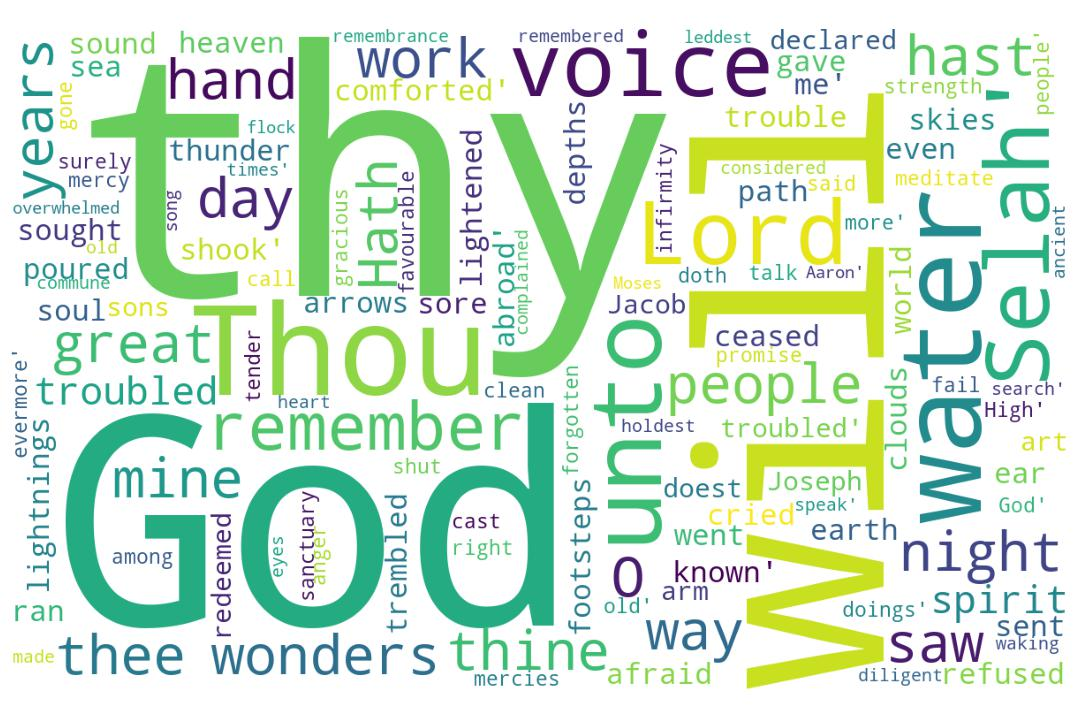
\includegraphics[width=\linewidth]{19OT-Psalms/Psalm77-WordCloud.jpg}
  \caption{Psalm 77 Word Cloud}
  \label{fig:Psalm 77 Word Cloud}
\end{figure}

\marginpar{\scriptsize \centering \fcolorbox{bone}{lime}{\textbf{GOD IS $\hdots$}}\\ (Psalm 77) \begin{compactenum}[I.][8]
    \item \textbf{My Silence} \index[scripture]{Psalms!Psa 077:04}(Psa 77:4)
    \item \textbf{My Searching} \index[scripture]{Psalms!Psa 077:06}(Psa 77:6)
    \item \textbf{My Song} \index[scripture]{Psalms!Psa 077:06}(Psa 77:6)
    \item \textbf{My Spech} \index[scripture]{Psalms!Psa 077:12}(Psa 77:12)
    \item \textbf{My Strength} \index[scripture]{Psalms!Psa 077:14}(Psa 77:14)
    \item \textbf{My Salvation} \index[scripture]{Psalms!Psa 077:15}(Psa 77:15)
    \item \textbf{My Saviour} \index[scripture]{Psalms!Psa 077:20}(Psa 77:20)
\end{compactenum}}
    

\marginpar{\scriptsize \centering \fcolorbox{bone}{yellow}{\textbf{A CHANGE OF}}\\
\fcolorbox{bone}{yellow}{\textbf{HEART AND MIND}}\\ (Psalm 77) 
\begin{compactenum}[I.][8]
    \item \textbf{There is Complaining} \index[scripture]{Psalms!Psa 077:03}(Psa 77:3)
    \item \textbf{There is Considering} \index[scripture]{Psalms!Psa 077:05}(Psa 77:5)
    \item \textbf{There is Communing with your Heart} \index[scripture]{Psalms!Psa 077:06}(Psa 77:6)
    \item \textbf{Thinking God Could Cast off his People} \index[scripture]{Psalms!Psa 077:07}(Psa 77:7)
    \item \textbf{But then Calling to Mind (remembering)} \index[scripture]{Psalms!Psa 077:11}(Psa 77:11)
    \item \textbf{And then God Confounds us} \index[scripture]{Psalms!Psa 077:13}(Psa 77:13) with his greatness, goodness, grace ...
    \item \textbf{That we can barely Contemplate Him} \index[scripture]{Psalms!Psa 077:14}(Psa 77:14)
\end{compactenum}}

\marginpar{\scriptsize \centering \fcolorbox{bone}{black}{\textbf{\textcolor{white}{THE PATH TO}}}\\ \fcolorbox{bone}{black}{\textbf{\textcolor{white}{DELIVERANCE}}}\\(Psalm 77) \begin{compactenum}[I.][8]
    \item \textbf{Revulsion} \index[scripture]{Psalms!Psa 077:02}(Psa 77:2)
    \item \textbf{Refusal} \index[scripture]{Psalms!Psa 077:03}(Psa 77:3)
    \item \textbf{Remembering} \index[scripture]{Psalms!Psa 077:03}\index[scripture]{Psalms!Psa 077:06}\index[scripture]{Psalms!Psa 077:11}\index[scripture]{Psalms!Psa 077:06}(Psa 77:3, 6, 10, 11)
    \item \textbf{Result} \index[scripture]{Psalms!Psa 077:10}(Psa 77:10)
    \item \textbf{Realization} \index[scripture]{Psalms!Psa 077:10}\index[scripture]{Psalms!Psa 077:13}(Psa 77:10, 13)
    \item \textbf{Redemption} \index[scripture]{Psalms!Psa 077:15}(Psa 77:15)
    \item \textbf{Revelation} \index[scripture]{Psalms!Psa 077:18}(Psa 77:18)
    \item \textbf{Rescue} \index[scripture]{Psalms!Psa 077:20}(Psa 77:20)
\end{compactenum}}


% \textcolor[cmyk]{0.99998,1,0,0}{
\footnote{\textcolor[rgb]{0.00,0.25,0.00}{\hyperlink{TOC}{Return to end of Table of Contents.}}}\footnote{\href{https://audiobible.com/bible/psalms_77.html}{\textcolor[cmyk]{0.99998,1,0,0}{Psalm 77 Audio}}}\textcolor[cmyk]{0.99998,1,0,0}{To the chief Musician, to Jeduthun, A Psalm of Asaph.}\\
\\
\textcolor[cmyk]{0.99998,1,0,0}{\fcolorbox{bone}{bone}{I} cried unto God with my voice, \emph{even} unto God with my voice; and he gave ear unto me.}
[2] \textcolor[cmyk]{0.99998,1,0,0}{In the day of my trouble \fcolorbox{bone}{bone}{I} sought the Lord: my sore ran in the night, and ceased not: my soul refused to be comforted.}\footnote{\textbf{Psalm 38:7} - For my loins are filled with a loathsome disease: and there is no soundness in my flesh.}
[3] \textcolor[cmyk]{0.99998,1,0,0}{\fcolorbox{bone}{bone}{I} remembered God, and was troubled: \fcolorbox{bone}{bone}{I} complained, and my spirit was overwhelmed. \fcolorbox{bone}{red}{\textcolor{white}{Selah}}.}
[4] \textcolor[cmyk]{0.99998,1,0,0}{Thou holdest mine eyes waking: \fcolorbox{bone}{bone}{I} am so troubled that \fcolorbox{bone}{bone}{I} cannot speak.}
[5] \textcolor[cmyk]{0.99998,1,0,0}{\fcolorbox{bone}{bone}{I} have considered the days of old, the years of ancient times.}\footnote{\textbf{Isaiah 46:10} - Declaring the end from the beginning, and from ancient times the things that are not yet done, saying, My counsel shall stand, and I will do all my pleasure:}
[6] \textcolor[cmyk]{0.99998,1,0,0}{\fcolorbox{bone}{bone}{I} call to remembrance my song in the night: \fcolorbox{bone}{bone}{I} commune with mine own heart: and my spirit made diligent search.}
[7] \textcolor[cmyk]{0.99998,1,0,0}{Will the Lord cast off for ever? and will he be favourable no more?}
[8] \textcolor[cmyk]{0.99998,1,0,0}{Is his mercy clean gone for ever? doth \emph{his} promise fail for evermore?}\footnote{\textbf{1 Kings 8:56} - Blessed be the LORD, that hath given rest unto his people Israel, according to all that he promised: there hath not failed one word of all his good promise, which he promised by the hand of Moses his servant.}
[9] \textcolor[cmyk]{0.99998,1,0,0}{Hath God forgotten to be gracious? hath he in anger shut up his tender mercies? \fcolorbox{bone}{red}{\textcolor{white}{Selah}}.}
[10] \textcolor[cmyk]{0.99998,1,0,0}{And \fcolorbox{bone}{bone}{I} said, This \emph{is} my infirmity: \emph{but} \emph{I} \emph{will} \emph{remember} the years of the right hand of the most High.}
[11] \textcolor[cmyk]{0.99998,1,0,0}{\fcolorbox{bone}{bone}{I} will remember the works of the LORD: surely \fcolorbox{bone}{bone}{I} will remember thy wonders of old.}
[12] \textcolor[cmyk]{0.99998,1,0,0}{\fcolorbox{bone}{bone}{I} will meditate also of all thy work, and talk of thy doings.}
[13] \textcolor[cmyk]{0.99998,1,0,0}{Thy way, O God, \emph{is} in the sanctuary: who \emph{is} \emph{so} great a God as \emph{our} God?}
[14] \textcolor[cmyk]{0.99998,1,0,0}{Thou \emph{art} the God that doest wonders: thou hast declared thy strength among the people.}
[15] \textcolor[cmyk]{0.99998,1,0,0}{Thou hast with \emph{thine} arm redeemed thy people, the sons of Jacob and Joseph. \fcolorbox{bone}{red}{\textcolor{white}{Selah}}.}
[16] \textcolor[cmyk]{0.99998,1,0,0}{The waters saw thee, O God, the waters saw thee; they were afraid: the depths also were troubled.}\footnote{\textbf{Job 41:32-32} - He maketh the deep to boil like a pot: he maketh the sea like a pot of ointment. [32] He maketh a path to shine after him; one would think the deep to be hoary. }\footnote{\textbf{Psalm 68:22} - The Lord said, I will bring again from Bashan, I will bring my people again from the depths of the sea:}
[17] \textcolor[cmyk]{0.99998,1,0,0}{The clouds poured out water: the skies sent out a sound: thine arrows also went abroad.}\footnote{\textbf{Psalm 18:14} - Yea, he sent out his arrows, and scattered them; and he shot out lightnings, and discomfited them.}\footnote{\textbf{Habakkuk 3:11} - The sun and moon stood still in their habitation: at the light of thine arrows they went, and at the shining of thy glittering spear}
[18] \textcolor[cmyk]{0.99998,1,0,0}{The voice of thy thunder \emph{was} in the heaven: the lightnings lightened the world: the earth trembled and shook.}
[19] \textcolor[cmyk]{0.99998,1,0,0}{Thy way \emph{is} in the sea, and thy path in the great waters, and thy footsteps are not known.}
[20] \textcolor[cmyk]{0.99998,1,0,0}{Thou leddest thy people like a flock by the hand of Moses and Aaron.}


\chapter{Proverb 18}
\begin{figure}
  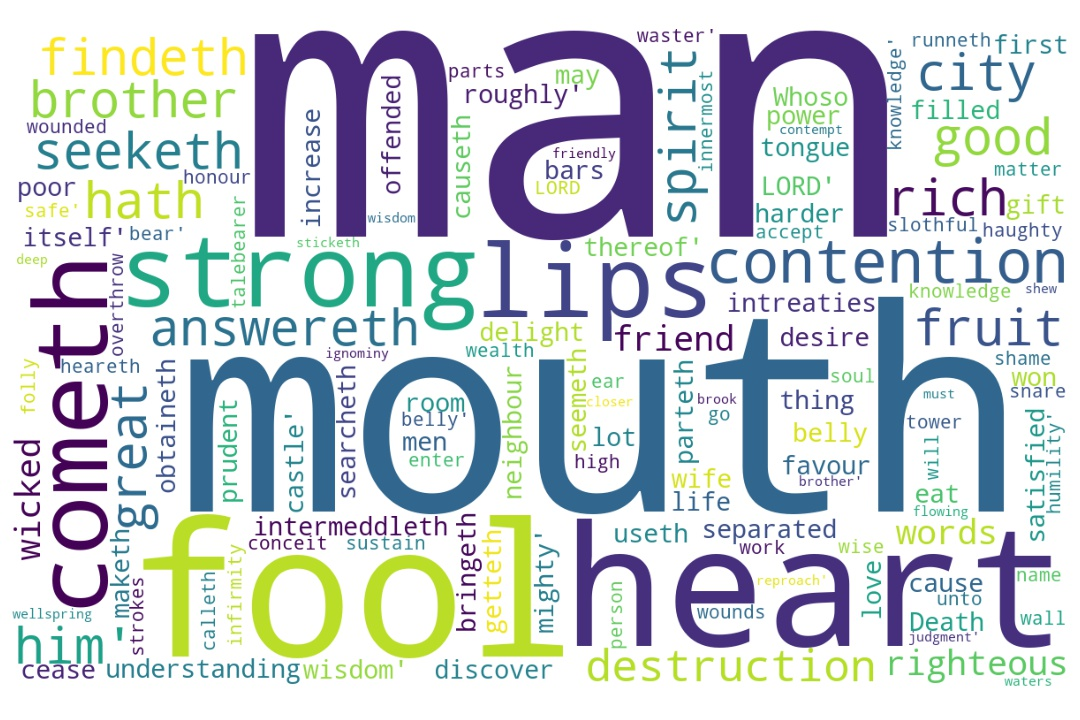
\includegraphics[width=\linewidth]{20OT-Proverbs/Proverb18-WordCloud.jpg}
  \caption{Proverb 18 Word Cloud}
  \label{fig:Proverb 18 word Cloud}
\end{figure}

\marginpar{\scriptsize \centering \fcolorbox{bone}{lime}{\textbf{A MAN FOCUSED ON GOD}}\\ (Proverbs 18:1-24) \begin{compactenum}[I.][8]
    \item Will be an \textbf{Inspired Man} - 
    \item Will be \textbf{Separate from the Ignorant Masses} - 
    \item For him most things in life will have  
    \textbf{Insignificant Meaning} - 
    \item Lives in an \textbf{Isolated Manner} 
    \item Lives by an \textbf{Individual Mandate} 
    \item Has an \textbf{intense and Insular Mentality}
\end{compactenum}}

\marginpar{\scriptsize \centering \fcolorbox{bone}{yellow}{\textbf{A FRIEND LIKE JESUS}}\\ (Proverb 18:24) \begin{compactenum}[I.][8]
    \item A \textbf{Close} Friend
    \item A \textbf{Constant} Friend
    \item A \textbf{Confiding} Friend
    \item A \textbf{Concerned} Friend
    \item A \textbf{Continuing} Friend
    \item A \textbf{Capable} Friend
    \item A \textbf{Caring} Friend
\end{compactenum}}

\marginpar{\scriptsize \centering \fcolorbox{bone}{black}{\textbf{\textcolor{white}{THE PURSUIT OF WISDOM}}}\\ (Proverb 18:24) \begin{compactenum}[I.][8]
    \item Then \textbf{Perverted} Motive -- to learn how manipulate events and circumstances. \index[scripture]{Proverbs!Pro 18:01}(Proverb 18:1)
    \item Then \textbf{Prideful} Motive -- To become exalted as wise. 
    \item Then \textbf{Public} Motive -- to be known and famous. 
    \item Then \textbf{Personal} Motive -- to achieve understanding. 
    \item Then \textbf{Practical} Motive -- to learn how live without mistakes or errors. 
    \item Then \textbf{Purposeful} Motive -- to learn navigate a specific problem. 
    \item Then \textbf{Perfect} Motive -- to learn how to live righteously before God. 
\end{compactenum}}

\marginpar{\scriptsize \centering \fcolorbox{bone}{blue}{\textbf{\textcolor{white}{WHAT YOUR SPEECH REVEALS}}}\\ (Proverb 18:4) \begin{compactenum}[I.][8]
    \item \textbf{Your Education} 
    \item \textbf{Your Excellence} 
    \item \textbf{Your Excitements} 
    \item \textbf{Your Enmity} 
    \item \textbf{Your Enemies} 
    \item \textbf{Your End} 
    \item \textbf{Your Emptiness}
    \item \textbf{Your Entanglements} 
\end{compactenum} }

\marginpar{\scriptsize \centering \fcolorbox{bone}{orange}{\textbf{THE WISE MAN}}\\ (Proverbs 18:1-24) \begin{compactenum}[I.][8]
    \item \textbf{Is Distinctive}
    \item \textbf{Is Disciplined}
    \item \textbf{Ignores Distractions}
    \item \textbf{Finds Delights in Wisdom}
    \item \textbf{Has Departed from the Common and Mundane}
    \item \textbf{Has a Distaste for Foolishness}
    \item \textbf{Is often regarded as Disturbed}
\end{compactenum} }




\footnote{\textcolor[cmyk]{0.99998,1,0,0}{\hyperlink{TOC}{Return to end of Table of Contents.}}}\footnote{\href{https://audiobible.com/bible/proverbs_18.html}{\textcolor[cmyk]{0.99998,1,0,0}{Proverbs Audio}}}\textcolor[cmyk]{0.99998,1,0,0}{Through desire a man, having separated himself, seeketh \emph{and} \fcolorbox{bone}{MYGOLD}{intermeddleth} with all wisdom.}
[2] \textcolor[cmyk]{0.99998,1,0,0}{A fool hath no delight in \fcolorbox{bone}{MYGOLD}{understanding}, but that \fcolorbox{bone}{bone}{his} heart may discover itself.}
[3] \textcolor[cmyk]{0.99998,1,0,0}{When the wicked cometh, \emph{then} cometh also contempt, and with ignominy reproach.}
[4] \textcolor[cmyk]{0.99998,1,0,0}{The words of a man's mouth \emph{are} \emph{as} deep waters, \emph{and} the wellspring of wisdom \emph{as} a flowing brook.}\footnote{\textbf{Proverb 16:22} - Understanding is a wellspring of life unto him that hath it: but the instruction of fools is folly.}
[5] \textcolor[cmyk]{0.99998,1,0,0}{\emph{It} \emph{is} not good to accept the person of the wicked, to overthrow the righteous in judgment.}
[6] \textcolor[cmyk]{0.99998,1,0,0}{A fool's lips enter into contention, and \fcolorbox{bone}{bone}{his} mouth calleth for strokes.}
[7] \textcolor[cmyk]{0.99998,1,0,0}{A fool's mouth \emph{is} \fcolorbox{bone}{bone}{his} destruction, and \fcolorbox{bone}{bone}{his} lips \emph{are} the snare of \fcolorbox{bone}{bone}{his} soul.}
[8] \textcolor[cmyk]{0.99998,1,0,0}{The words of a talebearer \emph{are} as wounds, and they go down into the innermost parts of the belly.}
[9] \textcolor[cmyk]{0.99998,1,0,0}{He also that is slothful in \fcolorbox{bone}{bone}{his} work is brother to him that is a great waster.}
[10] \textcolor[cmyk]{0.99998,1,0,0}{The name of the LORD \emph{is} a strong tower: the righteous runneth into it, and is safe.}
[11] \textcolor[cmyk]{0.99998,1,0,0}{The rich man's wealth \emph{is} \fcolorbox{bone}{bone}{his} strong city, and as an high wall in \fcolorbox{bone}{bone}{his} own conceit.}
[12] \textcolor[cmyk]{0.99998,1,0,0}{Before destruction the heart of man is haughty, and before honour \emph{is} humility.}
[13] \textcolor[cmyk]{0.99998,1,0,0}{He that answereth a matter before he heareth \emph{it}, it \emph{is} folly and shame unto him.}
[14] \textcolor[cmyk]{0.99998,1,0,0}{The spirit of a man will sustain \fcolorbox{bone}{bone}{his} infirmity; but a wounded spirit who can bear?}
[15] \textcolor[cmyk]{0.99998,1,0,0}{The heart of the prudent getteth knowledge; and the ear of the wise seeketh knowledge.}
[16] \textcolor[cmyk]{0.99998,1,0,0}{A man's gift maketh room for him, and bringeth him before great men.}
[17] \textcolor[cmyk]{0.99998,1,0,0}{\emph{He} \emph{that} \emph{is} first in \fcolorbox{bone}{bone}{his} own cause \emph{seemeth} just; but \fcolorbox{bone}{bone}{his} neighbour cometh and searcheth him.}
[18] \textcolor[cmyk]{0.99998,1,0,0}{The lot causeth contentions to cease, and parteth between the mighty.}
[19] \textcolor[cmyk]{0.99998,1,0,0}{A brother offended \emph{is} \emph{harder} \emph{to} \emph{be} \emph{won} than a strong city: and \emph{their} contentions \emph{are} like the bars of a castle.}
[20] \textcolor[cmyk]{0.99998,1,0,0}{A man's belly shall be satisfied with the fruit of \fcolorbox{bone}{bone}{his} mouth; \emph{and} with the increase of \fcolorbox{bone}{bone}{his} lips shall he be filled.}
[21] \textcolor[cmyk]{0.99998,1,0,0}{Death and life \emph{are} in the power of the tongue: and they that love it shall eat the fruit thereof.}
[22] \textcolor[cmyk]{0.99998,1,0,0}{\emph{Whoso} findeth a wife findeth a good \emph{thing}, and obtaineth favour of the LORD.}
[23] \textcolor[cmyk]{0.99998,1,0,0}{The poor useth intreaties; but the rich answereth roughly.}
[24] \textcolor[cmyk]{0.99998,1,0,0}{A man \emph{that} \emph{hath} friends must shew himself friendly: and there is a friend \emph{that} sticketh closer than a brother.}




\end{document}

